
\documentclass[11pt]{article}
\usepackage[margin=1in]{geometry}
\usepackage{booktabs}
\usepackage{longtable}
\usepackage{array}
\usepackage{graphicx}
\usepackage{siunitx}
\usepackage{tikz}
\usetikzlibrary{positioning,arrows.meta}
\usepackage{hyperref}
\usepackage{float}
\usepackage{xcolor}
\title{Solar Plane Design Report (Detailed, with MPPT + Graphs)}
\author{Project workspace: C:\textbackslash Users\textbackslash Janal\textbackslash NewPWS}
\date{\today}

\begin{document}
\maketitle

\section*{1. Project Inputs and Constraints}
\begin{itemize}
  \item Airframe mass used in analysis: \SI{1.851}{kg} (your \SI{1.70}{kg} baseline plus servos, wiring, MPPT allowance).
  \item Wing geometry: span \SI{3.00}{m}, area \SI{0.600}{m^2}, aspect ratio 15.00.
  \item Solar cells: 21 cells of \SI{125}{mm} x \SI{125}{mm} mono.
  \item Battery bay hard limits: depth \SI{54}{mm}, width \SI{31}{mm} (+\SI{3}{mm} tolerated), height \SI{19}{mm}.
  \item Existing propulsion hardware: D3530 1100KV, 14x4.7 slow-fly prop (CW), 50A ESC.
\end{itemize}
\subsection*{Chosen control/telemetry chain (user-selected)}
\begin{itemize}
  \item SpeedyBee F405
  \item UART MAVLink link to Raspberry Pi Zero 2 W
  \item mavlink-router on Pi
  \item A7670 LTE modem for WAN uplink
  \item Internet tunnel to QGroundControl
\end{itemize}
\begin{itemize}
  \item Avionics power included in calculations: FC \SI{1.0}{W} + Pi \SI{1.8}{W} + LTE modem avg \SI{3.0}{W} + misc \SI{0.5}{W} = \SI{6.3}{W}.
  \item Compatibility check: UART level is 3.3V on Pi GPIO UART and typical FC UART logic, so direct serial data interface is valid when grounds are shared.
  \item Risk 1 (power): A7670-class LTE modules have high TX current pulses; do not power the modem from Pi 5V pin. Use a dedicated regulator and local bulk capacitance.
  \item Risk 2 (control): cellular latency/coverage can drop unexpectedly; keep ELRS as primary C2 and use LTE for telemetry/backup control path.
  \item Risk 3 (firmware headroom): F405 targets can be flash-limited for advanced ArduPilot feature sets; verify your exact target build fits required features before finalizing.
\end{itemize}

\section*{2. Core Performance Results}
\begin{itemize}
  \item Estimated stall speed: \SI{6.42}{m/s}
  \item Best-endurance speed: \SI{8.25}{m/s}
  \item Mission speed used (1.4 x stall margin): \SI{8.98}{m/s}
  \item Propulsion electrical power at best-endurance speed: \SI{17.95}{W}
  \item Total electrical power at best-endurance speed (propulsion + avionics): \SI{24.25}{W}
  \item Total electrical power at mission speed: \SI{27.71}{W} (propulsion \SI{21.41}{W} + avionics \SI{6.30}{W})
  \item Motor estimate: loaded RPM \SI{5417}{rpm}, current \SI{28.0}{A}, static thrust \SI{12.0}{N}
\end{itemize}

\section*{3. Flight Power and Duration Graphs}
\begin{figure}[H]
\centering
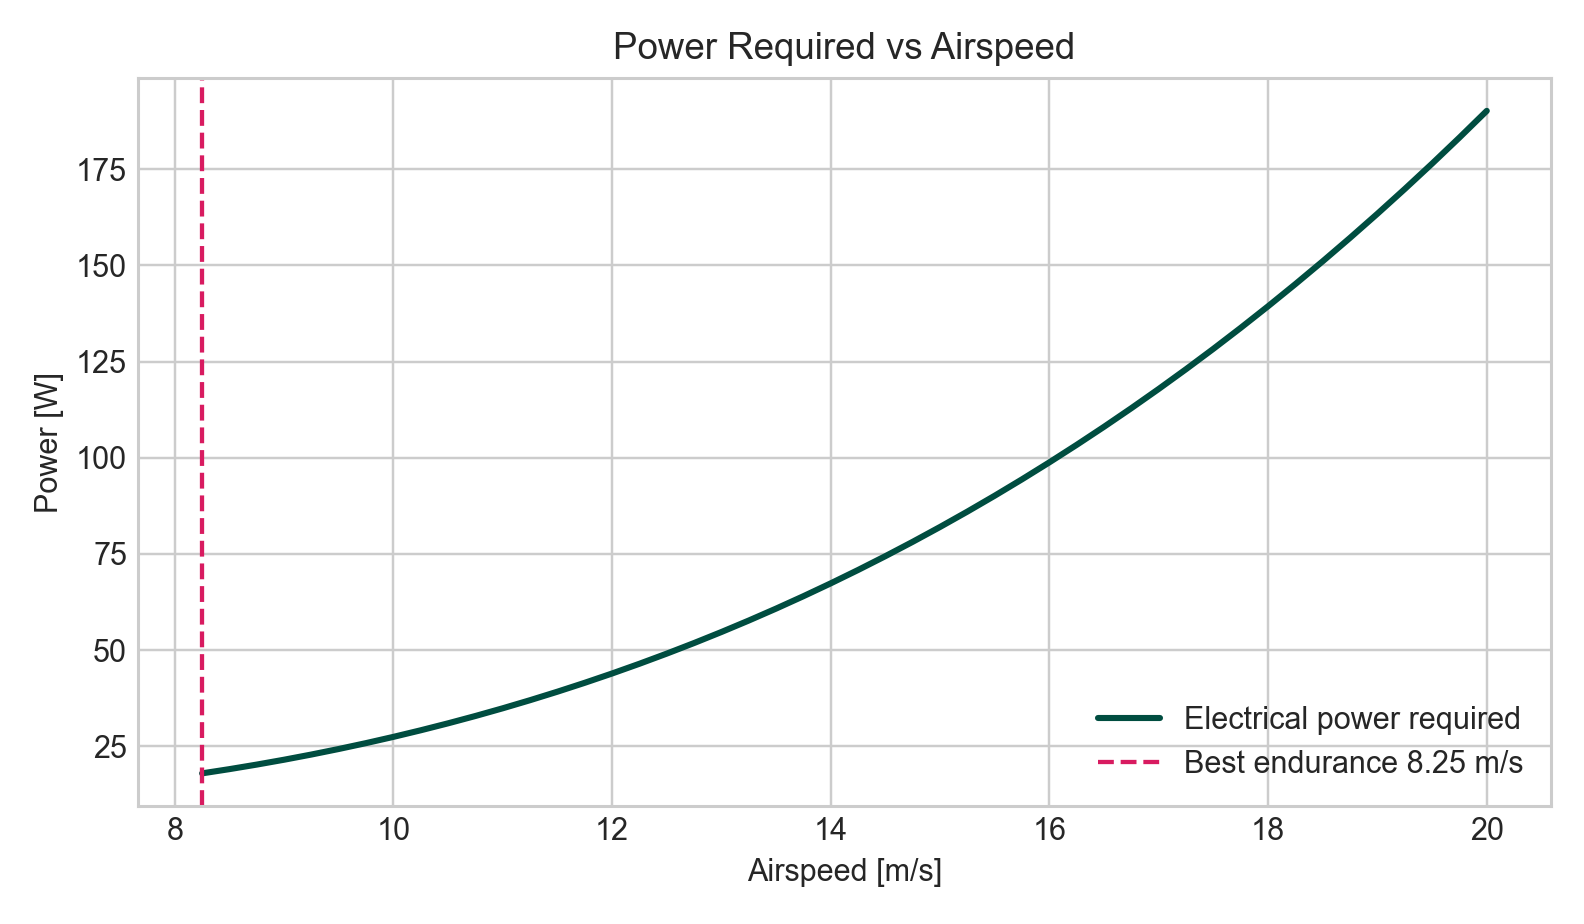
\includegraphics[width=0.9\linewidth]{figures/power_vs_speed.png}
\caption{Propulsion electrical power required vs airspeed.}
\end{figure}

\begin{figure}[H]
\centering
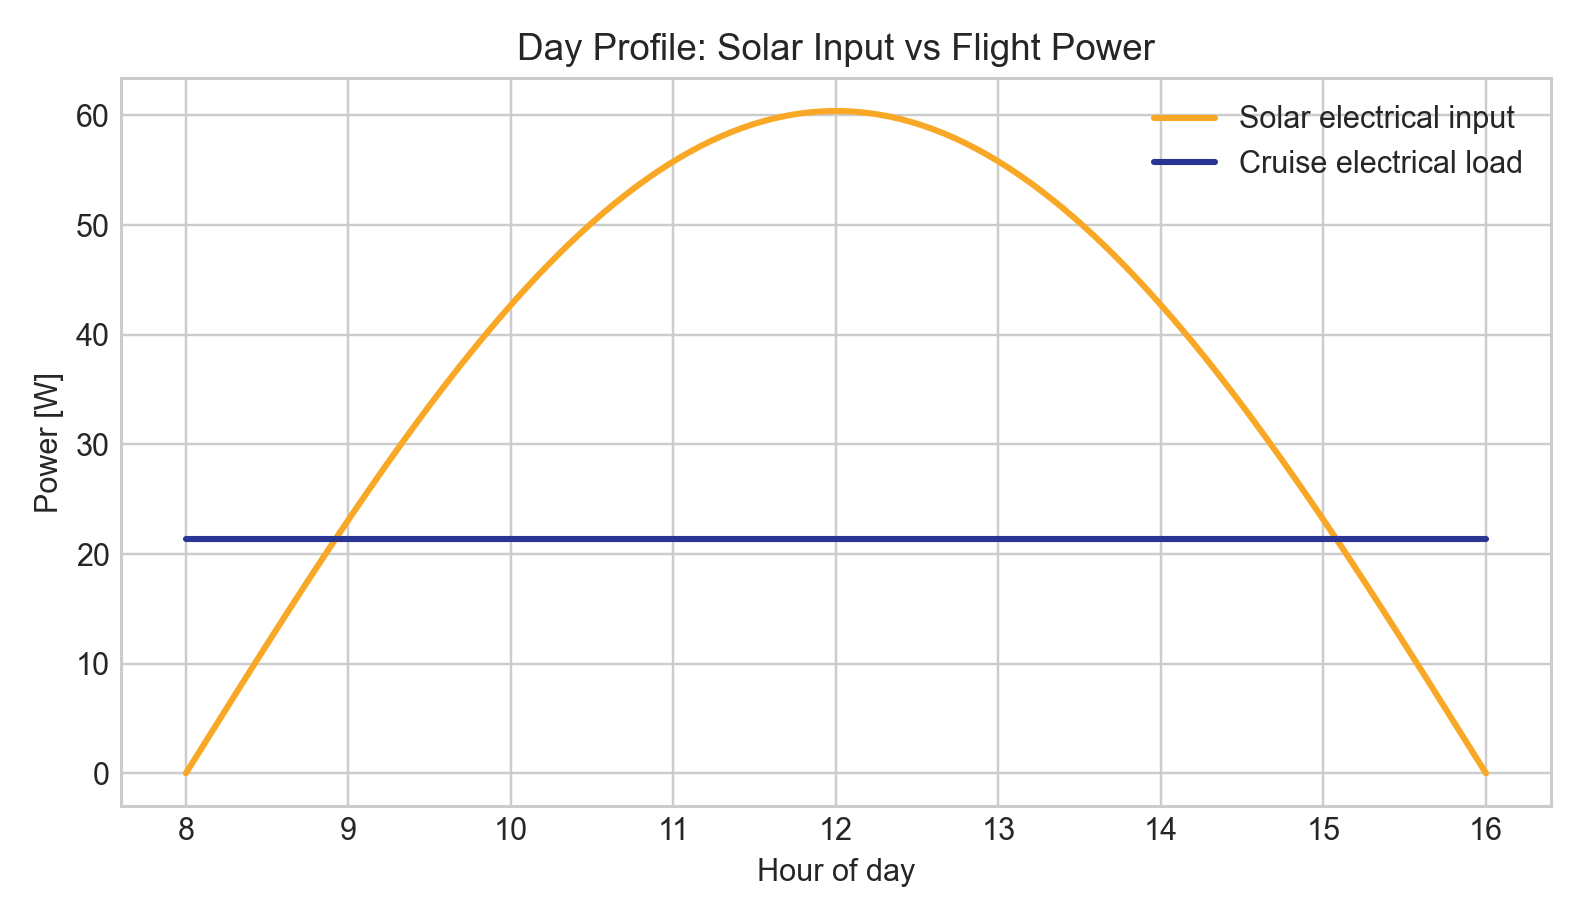
\includegraphics[width=0.9\linewidth]{figures/solar_vs_load.png}
\caption{Day profile power balance: solar input vs total cruise load (propulsion + avionics).}
\end{figure}

\begin{figure}[H]
\centering
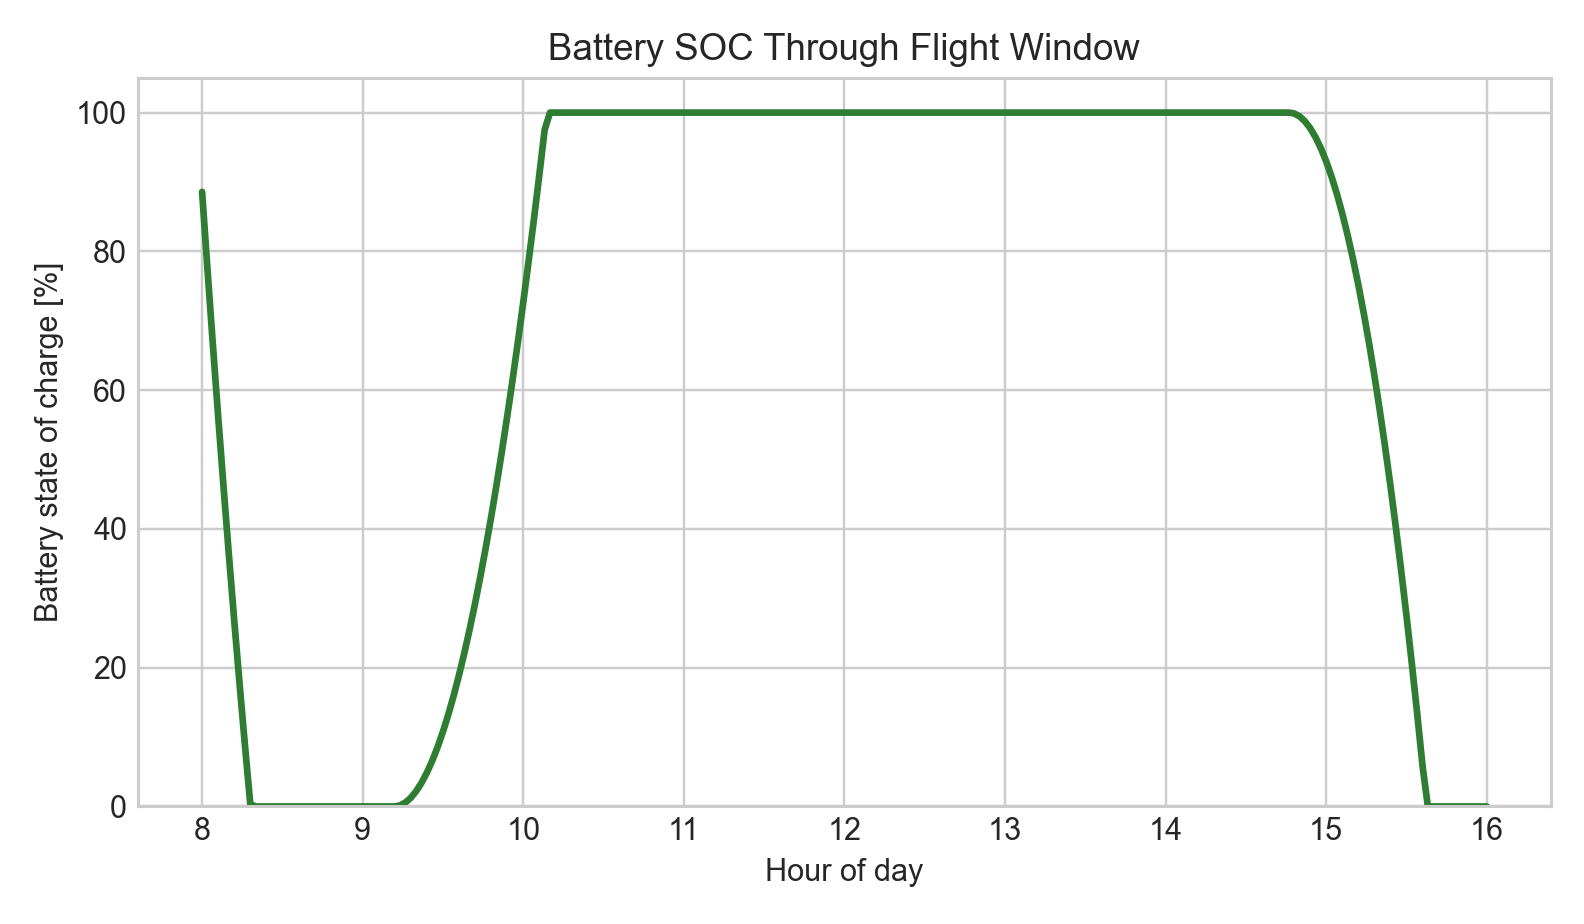
\includegraphics[width=0.9\linewidth]{figures/soc_vs_time.png}
\caption{Battery state of charge through the daylight mission window.}
\end{figure}

\begin{figure}[H]
\centering
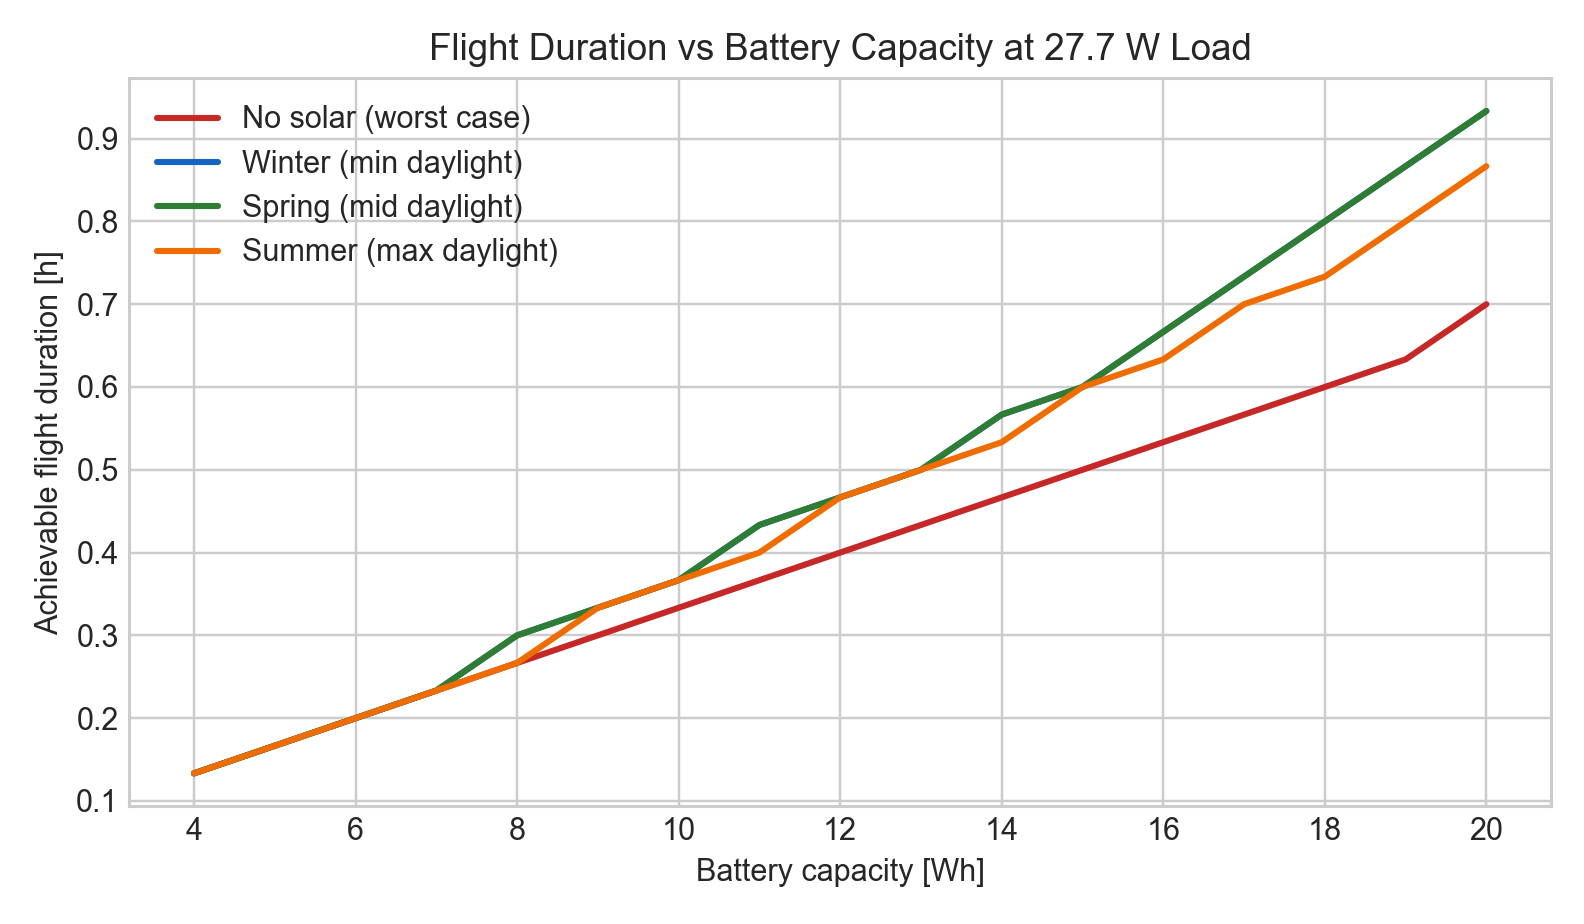
\includegraphics[width=0.9\linewidth]{figures/duration_vs_battery.png}
\caption{Flight duration versus battery capacity (with and without solar support).}
\end{figure}

\begin{figure}[H]
\centering
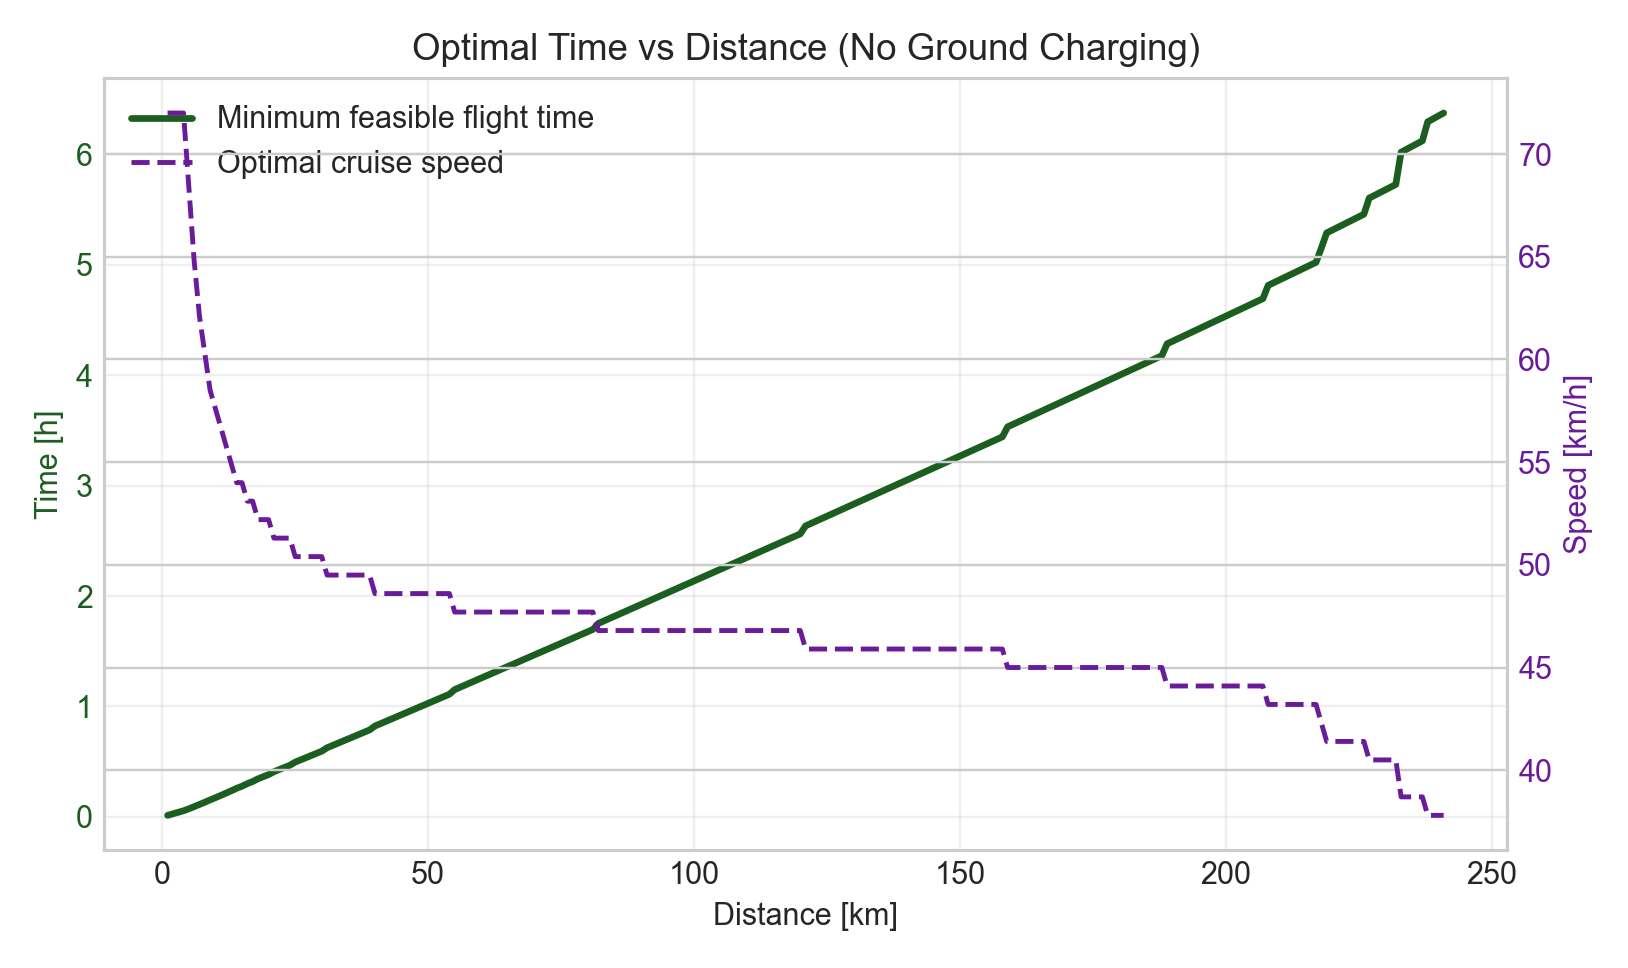
\includegraphics[width=0.92\linewidth]{figures/time_vs_distance_optimal.png}
\caption{Time vs distance envelope without ground charging. For each distance, speed and departure time are optimized to minimize total flight time.}
\end{figure}

\begin{figure}[H]
\centering
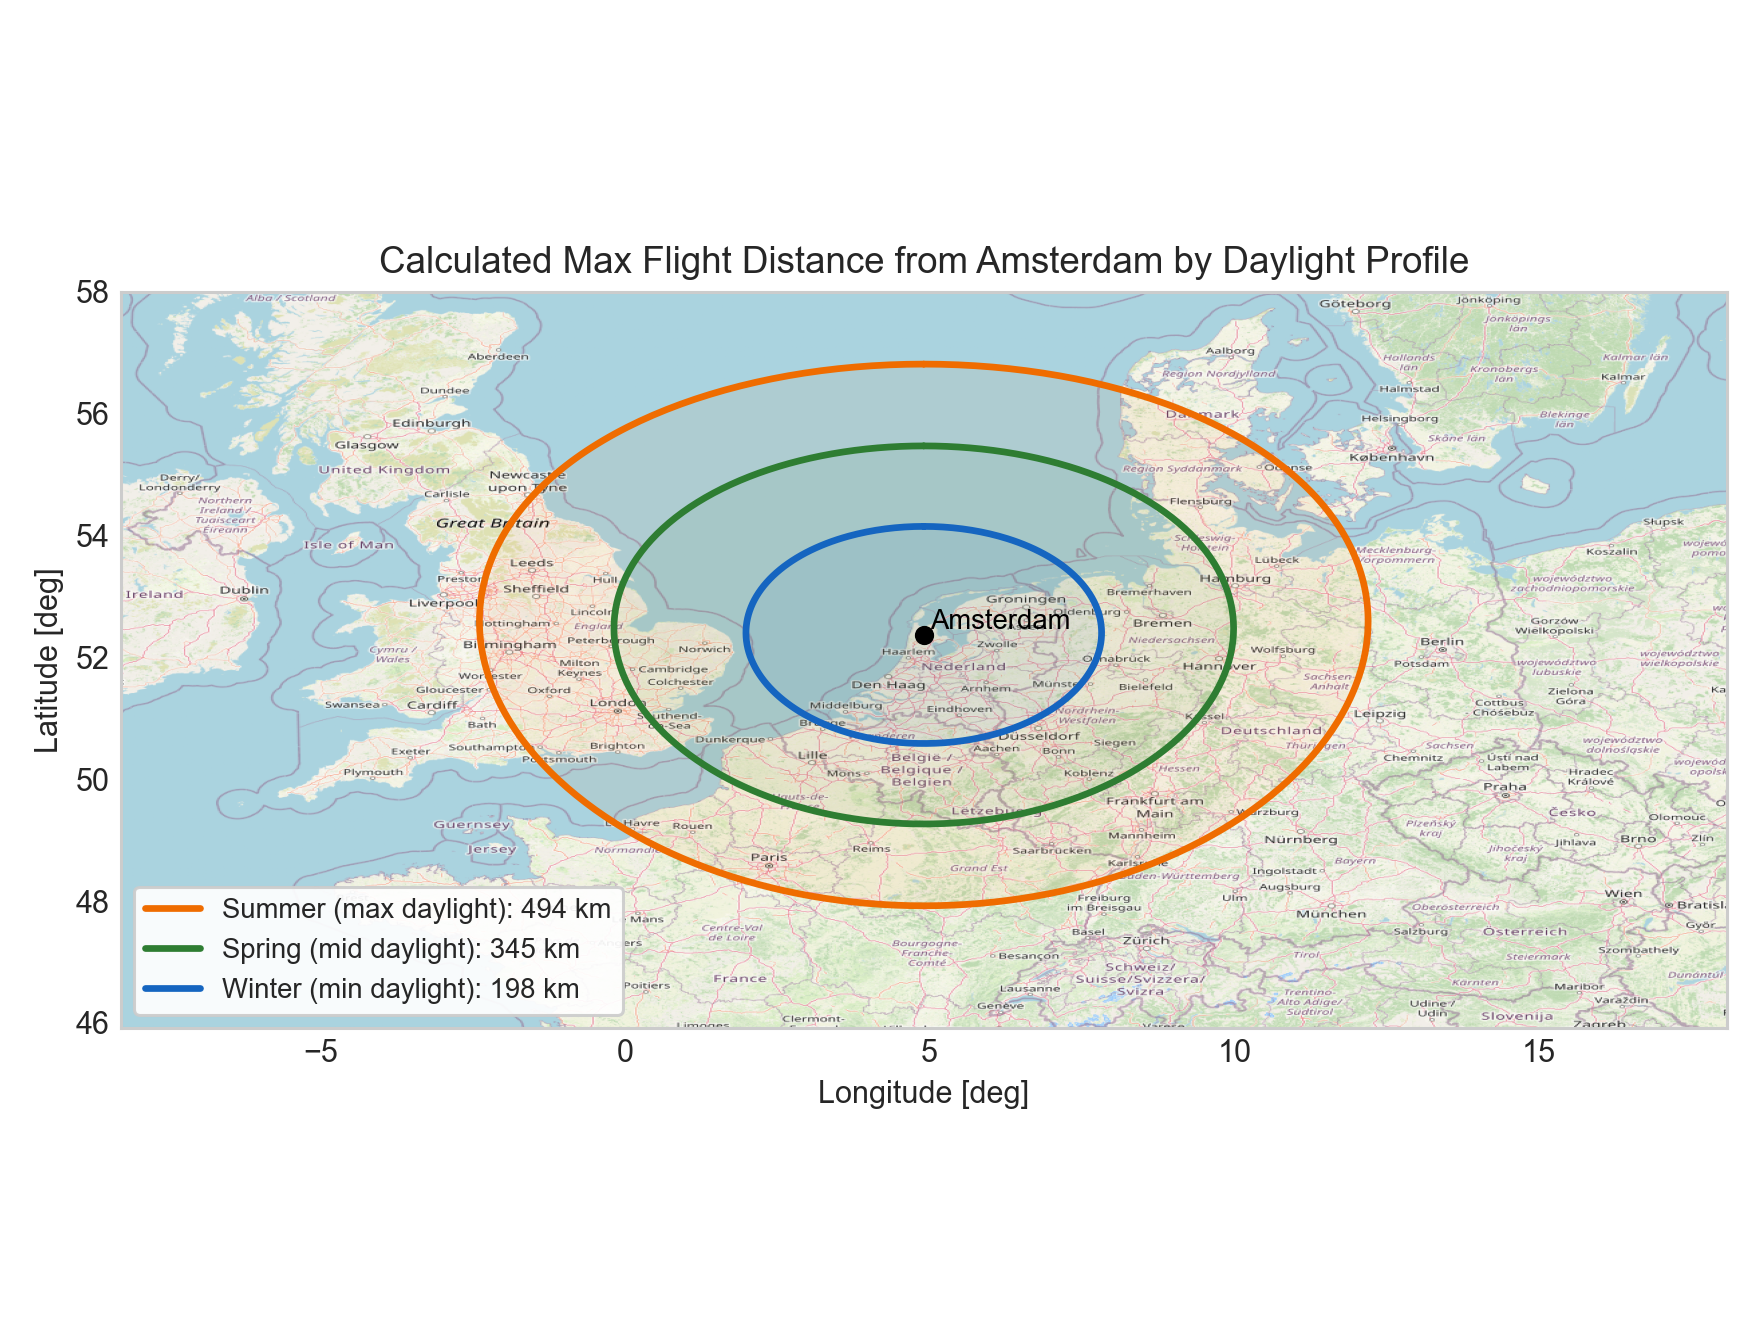
\includegraphics[width=0.92\linewidth]{figures/amsterdam_daylight_range_map.png}
\caption{Range circles centered on Amsterdam using the calculated maximum distance for winter (min), spring (mid), and summer (max) daylight profiles.}
\end{figure}

\textbf{Sample optimal points (no ground charging, battery starts at 100\% SOC):}
\begin{itemize}
\item 10 km: 0.17 h, optimal speed 57.6 km/h, optimal start 11.33h
\item 25 km: 0.50 h, optimal speed 50.4 km/h, optimal start 11.00h
\item 50 km: 1.03 h, optimal speed 48.6 km/h, optimal start 11.17h
\item 75 km: 1.57 h, optimal speed 47.7 km/h, optimal start 11.00h
\item 100 km: 2.14 h, optimal speed 46.8 km/h, optimal start 10.50h
\item 150 km: 3.27 h, optimal speed 45.9 km/h, optimal start 10.17h
\item 200 km: 4.54 h, optimal speed 44.1 km/h, optimal start 9.67h
\end{itemize}

\textbf{Daylight profile assumptions and max-distance results:}
\begin{itemize}
\item Winter (min daylight): daylight 7.75 h, peak irradiance 550 W/m$^2$, max distance 198.1 km (best speed 31.5 km/h, best start 9.50h).
\item Spring (mid daylight): daylight 12.00 h, peak irradiance 850 W/m$^2$, max distance 345.0 km (best speed 36.0 km/h, best start 8.00h).
\item Summer (max daylight): daylight 16.75 h, peak irradiance 1000 W/m$^2$, max distance 494.3 km (best speed 37.8 km/h, best start 7.17h).
\end{itemize}

\section*{4. Battery Feasibility for Your Battery Bay}
\begin{itemize}
  \item 30-minute reserve target: \SI{15.16}{Wh} (minimum \SI{1365}{mAh} at 3S nominal).
  \item 20-minute reserve target: \SI{10.10}{Wh}.
  \item Theoretical max energy in bay (450--550 Wh/L): \SI{14.31}{Wh} to \SI{17.49}{Wh}.
  \item Daylight simulation minimum SOC: 0.0\%, final SOC: 0.0\%, first empty time: 8.33h.
\end{itemize}

\subsection*{Researched battery options}
\begin{longtable}{p{5.8cm} r r r c c c}
\toprule
Pack & mAh & Wh & g & D x W x H (mm) & Strict fit & Meets 30-min reserve \\
\midrule
\endhead
Thunder Power Pro Lite V2 3S 500mAh 70C & 500 & 5.55 & 49 & 53x30x13 & Yes & No \\
Thunder Power Pro Lite V2 3S 750mAh 70C & 750 & 8.32 & 69 & 55x31x18 & No & No \\
Tattu R-Line 3S 650mAh 75C & 650 & 7.21 & 70 & 58x31x16 & No & No \\
Tattu R-Line 3S 850mAh 75C & 850 & 9.43 & 91 & 58x30x22 & No & No \\
\bottomrule
\end{longtable}

\textbf{Strict-fit options found:} Thunder Power Pro Lite V2 3S 500mAh 70C

\textbf{If depth can extend to about 58 mm:} Thunder Power Pro Lite V2 3S 500mAh 70C, Thunder Power Pro Lite V2 3S 750mAh 70C, Tattu R-Line 3S 650mAh 75C

\section*{5. Proper MPPT Controller Selection (Module-level, not chip-only)}
Using your 21-cell panel as one series string:
\[
V_{MP,array} \approx 21 \cdot 0.55 = 11.55\ \mathrm{V},\quad
V_{OC,array} \approx 21 \cdot 0.64 = 13.44\ \mathrm{V}
\]
This panel voltage is below robust buck-MPPT headroom for charging a 3S Li-ion pack at \SI{12.6}{V}.
For buck topologies, practical cell count is about 25 (minimum) to 28 (recommended margin).
Therefore, with 21 cells, a \textbf{boost or buck-boost MPPT} is the correct architecture.

\subsection*{Selected converter for this build}
\textbf{Selected MPPT/buck-boost charger:} TI BQ25798EVM
\begin{itemize}
  \item Topology: Buck-boost charger with MPPT support
  \item Charge profile: Configure for 3S Li-ion (12.6V CV) through I2C
  \item Key specs used in this design: 3.6-24V input, 1-4 cell battery support, up to 5A charging current
  \item Fit with 21-cell + 3S architecture: Yes; buck-boost handles panel voltage below and above battery charge voltage
\end{itemize}

\subsection*{Required supporting components around MPPT}
\begin{itemize}
  \item PV fuse near panel positive lead, sized around 1.25x panel Isc branch current.
  \item Dedicated MPPT-to-battery branch fuse (about 10A).
  \item Main battery fuse for propulsion branch (about 40A with your ESC/motor class).
  \item XT60 (or equivalent) connectors and 16--14 AWG wire on high-current paths.
\end{itemize}

\section*{6. Wiring Diagram A: Power Architecture}
\begin{figure}[H]
\centering
\resizebox{0.98\linewidth}{!}{%
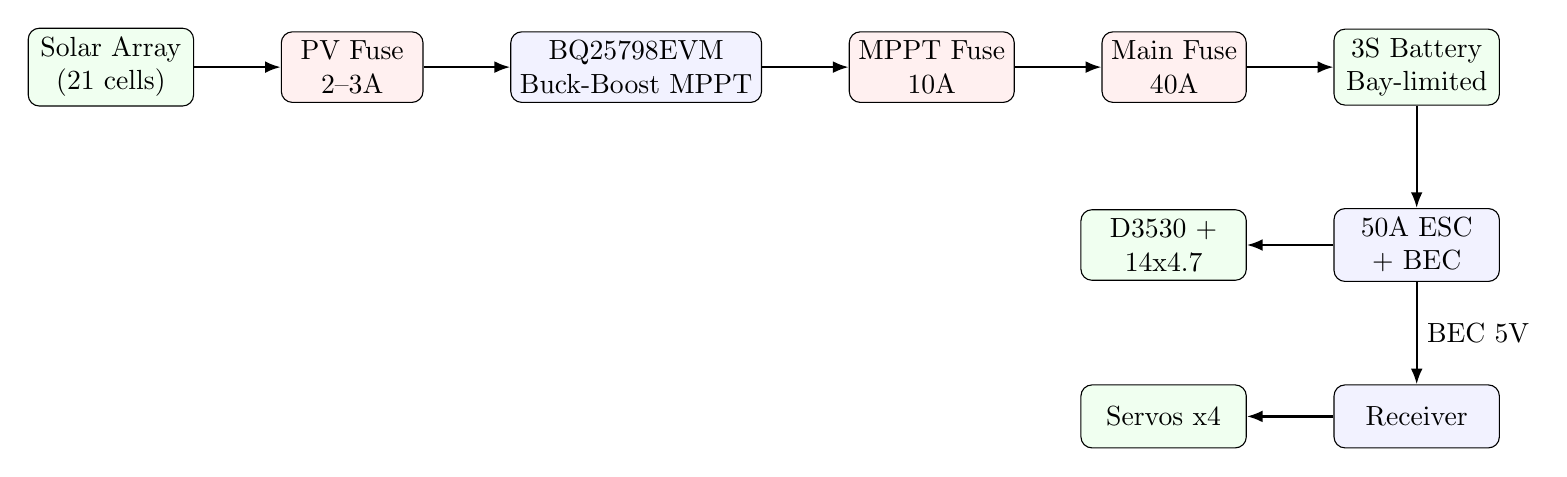
\begin{tikzpicture}[
    node distance=1.3cm and 1.1cm,
    block/.style={draw, rounded corners, align=center, minimum width=2.1cm, minimum height=0.8cm, fill=blue!5},
    io/.style={draw, rounded corners, align=center, minimum width=2.1cm, minimum height=0.8cm, fill=green!6},
    safety/.style={draw, rounded corners, align=center, minimum width=1.8cm, minimum height=0.8cm, fill=red!6},
    line/.style={-{Latex[length=2mm]}, thick}
]
\node[io] (solar) {Solar Array\\(21 cells)};
\node[safety, right=of solar] (sfuse) {PV Fuse\\2--3A};
\node[block, right=of sfuse] (mppt) {BQ25798EVM\\Buck-Boost MPPT};
\node[safety, right=of mppt] (mfuse) {MPPT Fuse\\10A};
\node[safety, right=of mfuse] (bfuse) {Main Fuse\\40A};
\node[io, right=of bfuse] (battery) {3S Battery\\Bay-limited};

\node[block, below=1.3cm of battery] (esc) {50A ESC\\+ BEC};
\node[io, left=of esc] (motor) {D3530 +\\14x4.7};
\node[block, below=1.3cm of esc] (rx) {Receiver};
\node[io, left=of rx] (servos) {Servos x4};

\draw[line] (solar) -- (sfuse);
\draw[line] (sfuse) -- (mppt);
\draw[line] (mppt) -- (mfuse);
\draw[line] (mfuse) -- (bfuse);
\draw[line] (bfuse) -- (battery);
\draw[line] (battery) -- (esc);
\draw[line] (esc) -- (motor);
\draw[line] (esc) -- node[right] {BEC 5V} (rx);
\draw[line] (rx) -- (servos);
\end{tikzpicture}
}
\caption{Recommended power wiring with dedicated MPPT branch protection.}
\end{figure}

\section*{7. Wiring Diagram B: Signal and Channel Mapping}
\begin{figure}[H]
\centering
\resizebox{0.92\linewidth}{!}{%
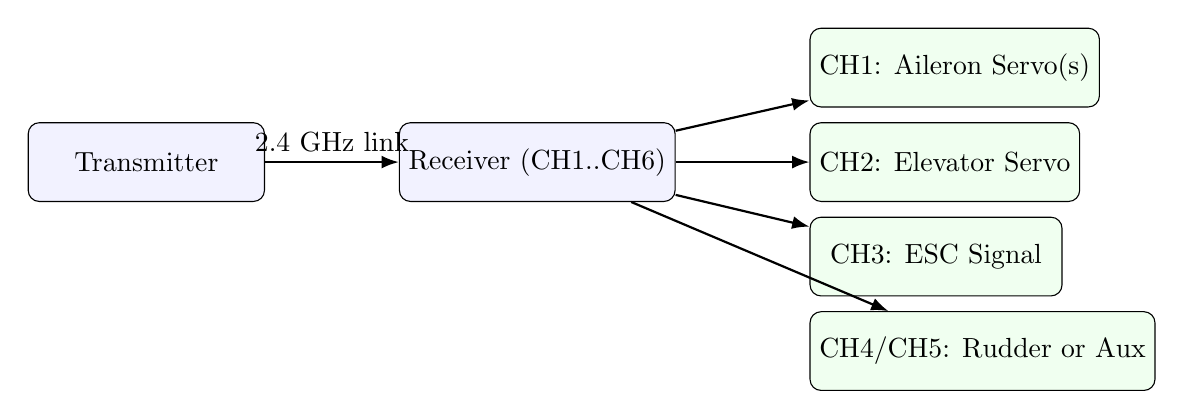
\begin{tikzpicture}[
    node distance=1.4cm and 1.7cm,
    block/.style={draw, rounded corners, align=center, minimum width=3.0cm, minimum height=1.0cm, fill=blue!5},
    io/.style={draw, rounded corners, align=center, minimum width=3.2cm, minimum height=1.0cm, fill=green!6},
    line/.style={-{Latex[length=2.2mm]}, thick}
]
\node[block] (tx) {Transmitter};
\node[block, right=of tx] (rx) {Receiver (CH1..CH6)};
\node[io, right=of rx, yshift=1.2cm] (ail) {CH1: Aileron Servo(s)};
\node[io, right=of rx, yshift=0.0cm] (elev) {CH2: Elevator Servo};
\node[io, right=of rx, yshift=-1.2cm] (thr) {CH3: ESC Signal};
\node[io, right=of rx, yshift=-2.4cm] (aux) {CH4/CH5: Rudder or Aux};

\draw[line] (tx) -- node[above] {2.4 GHz link} (rx);
\draw[line] (rx) -- (ail);
\draw[line] (rx) -- (elev);
\draw[line] (rx) -- (thr);
\draw[line] (rx) -- (aux);
\end{tikzpicture}
}
\caption{Signal wiring map. Verify channel assignments in transmitter before motor power-up.}
\end{figure}

\section*{8. Pin-level Wiring (Exact Connector Mapping)}
\subsection*{8.1 Shared power-bus rule}
Battery+, MPPT output+, and ESC+ are intentionally on the same positive DC bus node (through their branch fuses). Continuity between those + points is expected. A fault is only + to - continuity.

\subsection*{8.2 Receiver and ESC 3-wire lead pin mapping}
{\small
\begin{longtable}{>{\raggedright\arraybackslash}p{3.2cm} >{\raggedright\arraybackslash}p{2.0cm} >{\raggedright\arraybackslash}p{3.5cm} >{\raggedright\arraybackslash}p{3.5cm}}
\toprule
Wire color (typical) & Pin function & Connect to receiver pin row & Notes \\
\midrule
\endhead
White/Yellow/Orange & Signal (S) & CH3 signal pin & ESC throttle command line \\
Red & +5V BEC output & CH3 + pin (receiver power rail) & Powers receiver and servos if ESC has BEC \\
Black/Brown & Ground (GND) & CH3 - pin & Must share common ground with all RC signal devices \\
\bottomrule
\end{longtable}
}

\subsection*{8.3 Servo connector mapping}
{\small
\begin{longtable}{>{\raggedright\arraybackslash}p{2.4cm} >{\raggedright\arraybackslash}p{2.6cm} >{\raggedright\arraybackslash}p{3.8cm} >{\raggedright\arraybackslash}p{3.8cm}}
\toprule
Receiver channel & Control surface & Pin order on receiver & Typical wire colors \\
\midrule
\endhead
CH1 & Aileron & S / + / - & Orange or white / red / brown-black \\
CH2 & Elevator & S / + / - & Orange or white / red / brown-black \\
CH4 (optional) & Rudder & S / + / - & Orange or white / red / brown-black \\
CH5/CH6 (optional) & Aux, flaps, telemetry trigger & S / + / - & Orange or white / red / brown-black \\
\bottomrule
\end{longtable}
}

\subsection*{8.4 MPPT and high-current wiring map}
{\small
\begin{longtable}{>{\raggedright\arraybackslash}p{3.8cm} >{\raggedright\arraybackslash}p{3.2cm} >{\raggedright\arraybackslash}p{4.0cm}}
\toprule
Connection & Wire/fuse recommendation & Purpose \\
\midrule
\endhead
Solar+ to MPPT IN+ & PV fuse 2-3A near panel & Protect panel branch from short faults \\
MPPT OUT+ to battery bus+ & 10A fuse near battery bus & Protect charger branch and wiring \\
Battery bus+ to ESC+ & 40A main fuse near battery & Protect propulsion high-current branch \\
All negatives (solar/MPPT/battery/ESC) & Common ground return bus & Required for charger and RC signal reference \\
\bottomrule
\end{longtable}
}

\subsection*{8.5 Pre-power checklist}
\begin{enumerate}
  \item Remove propeller before bench wiring and ESC setup.
  \item Confirm no hard short between main bus + and - (ohmmeter should not read near-zero steady value).
  \item Confirm expected continuity between battery+, MPPT+, and ESC+ bus points.
  \item Power receiver/ESC first from battery only, verify channel directions.
  \item Connect solar and MPPT last, then confirm charging current with a wattmeter.
\end{enumerate}

\subsection*{8.6 Final companion-power wiring (exact implementation)}
\begin{itemize}
  \item Battery bus + -> branch fuse 2A -> D36V50F5 VIN.
  \item D36V50F5 VOUT 5V -> Pi Zero 2 W 5V (power input).
  \item Battery bus + -> branch fuse 3A -> D30V33MAL VIN.
  \item Set D30V33MAL VOUT = 4.0V before connecting modem.
  \item D30V33MAL VOUT 4.0V -> A7670 VBAT.
  \item A7670 GND, Pi GND, FC GND, battery - all tied together.
  \item SpeedyBee F405 UART TX/RX <-> Pi UART RX/TX (crossed), same GND.
  \item Pi USB/UART (per modem interface choice) -> A7670 data link.
\end{itemize}

\section*{9. Wiring Diagram C: Pin-level Connector Orientation}
\begin{figure}[H]
\centering
\resizebox{0.96\linewidth}{!}{%
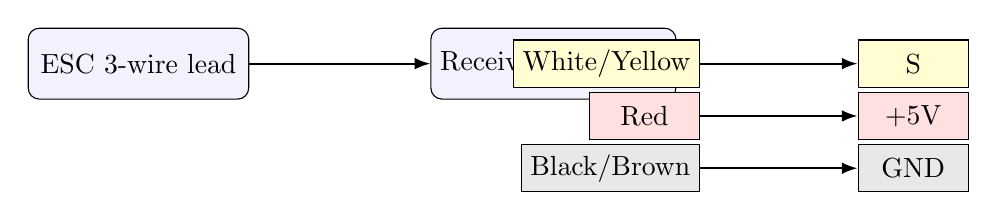
\begin{tikzpicture}[
    node distance=1.1cm and 1.2cm,
    box/.style={draw, rounded corners, align=center, minimum width=2.8cm, minimum height=0.9cm, fill=blue!5},
    pin/.style={draw, align=center, minimum width=1.4cm, minimum height=0.6cm},
    line/.style={-{Latex[length=2mm]}, thick}
]
\node[box] (rx) {Receiver CH3 port};
\node[pin, right=2.3cm of rx, fill=yellow!18] (sig) {S};
\node[pin, below=0.05cm of sig, fill=red!12] (vcc) {+5V};
\node[pin, below=0.05cm of vcc, fill=gray!18] (gnd) {GND};

\node[box, left=2.3cm of rx] (esclead) {ESC 3-wire lead};
\node[pin, left=2.0cm of sig, fill=yellow!18] (escsig) {White/Yellow};
\node[pin, left=2.0cm of vcc, fill=red!12] (escvcc) {Red};
\node[pin, left=2.0cm of gnd, fill=gray!18] (escgnd) {Black/Brown};

\draw[line] (esclead) -- (rx);
\draw[line] (escsig) -- (sig);
\draw[line] (escvcc) -- (vcc);
\draw[line] (escgnd) -- (gnd);
\end{tikzpicture}
}
\caption{ESC lead to receiver CH3 mapping. Keep signal, +5V and GND aligned in the same row orientation.}
\end{figure}

\section*{10. LW-PLA and Carbon Tube Build Notes}
\begin{itemize}
  \item LW-PLA should be printed hot enough for foaming expansion; tune flow down after expansion to reduce mass.
  \item Carbon tubes should carry main bending loads in wing spar caps or spar tube; printed parts should primarily transfer loads into tubes.
  \item Reinforce wing root and motor mount interfaces with local carbon doublers or thicker load-spreading printed inserts.
\end{itemize}

\section*{11. Sources}
\begin{enumerate}
  \item Solar cell electrical reference (CSE125P-6BB): \url{https://solarinnova.net/en/product/cell-cse125p-6bb/}
  \item TI BQ25798 product page (buck-boost charger with MPPT support): \url{https://www.ti.com/product/BQ25798}
  \item TI BQ25798 datasheet: \url{https://www.ti.com/lit/gpn/bq25798}
  \item TI BQ25798EVM user guide: \url{https://www.ti.com/lit/ug/sluucb5c/sluucb5c.pdf}
  \item TI BQ24650 datasheet: \url{https://www.ti.com/lit/gpn/bq24650}
  \item TI BQ24650 EVM user guide: \url{https://www.ti.com/lit/ug/sluu444a/sluu444a.pdf}
  \item SpeedyBee F405 product/target reference: \url{https://www.speedybee.com/speedybee-f405-wing-app-fixed-wing-flight-controller/}
  \item ArduPilot note on F4 flash constraints: \url{https://ardupilot.org/copter/docs/common-limited-firmware.html}
  \item SIMCom A7670 hardware design guide (power supply and burst current guidance): \url{https://simcom.ee/documents/A76XX/A76XX%20Series_Hardware%20Design_V1.07.pdf}
  \item MAVLink Router project/documentation: \url{https://github.com/mavlink-router/mavlink-router}
  \item QGroundControl project: \url{https://qgroundcontrol.com/}
  \item Thunder Power LiPo dimensions/spec chart: \url{https://www.chiefaircraft.com/downloads/tp-lipo.pdf}
  \item Tattu 650mAh 3S product page (dimensions): \url{https://www.gensace.de/tattu-r-line-650mah-11-1v-75c-3s1p-lipo-battery-pack-with-xt30-plug.html}
  \item Tattu 850mAh 3S product page (dimensions): \url{https://www.gensace.de/tattu-r-line-version-4-0-850mah-11-1v-75c-3s1p-lipo-battery-pack-with-xt30-plug.html}
  \item colorFabb LW-PLA product and print guidance: \url{https://colorfabb.com/lw-pla-natural?srsltid=AfmBOopoCdZegtz2AIdR2wfQZQ5N8a1ba9hLJxQFUnUGR92Ve8g7Qy2D}
  \item eSUN LW-PLA material data: \url{https://www.esun3d.com/epla-lw-product/}
  \item Easy Composites carbon tube data sheet: \url{https://www.easycomposites.co.uk/pub/media/pdf/carbon-fibre-tube-data-sheet.pdf}
  \item OpenStreetMap tile service: \url{https://tile.openstreetmap.org/}
\end{enumerate}

\end{document}
